% The delivery pad and the two-stage localization (TikZ), two panels with their labels below. Every size and position is
% make_pad.py's MARKERS and MAT; the radii are the landing tests of gz_learner.py (1.0 m) and wind/gz_windland.py (PAD_R 0.75 m).
\begin{figure*}[t]\centering
\begin{minipage}[b]{0.29\textwidth}\centering
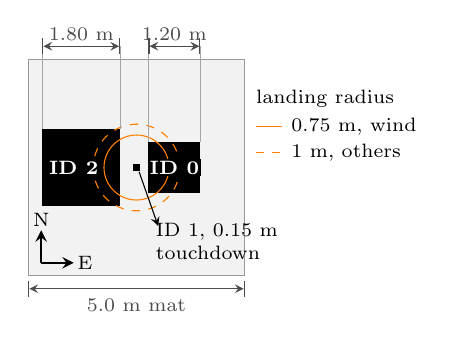
\begin{tikzpicture}[>=stealth, font=\scriptsize, x=0.55cm, y=0.55cm]
  \fill[black!5] (-2.5,-2.5) rectangle (2.5,2.5);
  \draw[black!40] (-2.5,-2.5) rectangle (2.5,2.5);
  \fill (-2.175,-0.9) rectangle (-0.375,0.9);                           % ID 2, 1.80 m, centre x = -1.275
  \fill (0.275,-0.6) rectangle (1.475,0.6);                             % ID 0, 1.20 m, centre x = +0.875
  \fill (-0.075,-0.075) rectangle (0.075,0.075);                        % ID 1, 0.15 m, at the origin
  \draw[orange] (0,0) circle (0.75);
  \draw[orange, dashed] (0,0) circle (1.0);
  \node[white, fill=black, inner sep=0.8pt, font=\scriptsize\bfseries] at (-1.45,0) {ID 2};
  \node[white, fill=black, inner sep=0.8pt, font=\scriptsize\bfseries] at (0.875,0) {ID 0};
  % sizes above the mat, on extension lines from the markers' corners
  \foreach \xa/\xb/\h in {-2.175/-0.375/0.9, 0.275/1.475/0.6} \draw[black!35, very thin] (\xa,\h) -- (\xa,2.8) (\xb,\h) -- (\xb,2.8);
  \draw[|<->|, black!70] (-2.175,2.8) -- node[above=2pt, inner sep=0pt] {1.80 m} (-0.375,2.8);
  \draw[|<->|, black!70] (0.275,2.8) -- node[above=2pt, inner sep=0pt] {1.20 m} (1.475,2.8);
  \draw[->] (0.06,-0.1) -- (0.5,-1.35) node[below right=-2pt, align=left, inner sep=1pt] {ID 1, 0.15 m\\touchdown};
  \draw[->, thick] (-2.2,-2.2) -- (-1.45,-2.2) node[right, inner sep=1pt] {E};
  \draw[->, thick] (-2.2,-2.2) -- (-2.2,-1.45) node[above, inner sep=1pt] {N};
  \draw[|<->|, black!70] (-2.5,-2.8) -- node[below] {5.0 m mat} (2.5,-2.8);
  \node[anchor=west, inner sep=0pt] at (2.75,1.6) {landing radius};
  \draw[orange] (2.75,0.95) -- (3.35,0.95) node[right, black] {0.75 m, wind};
  \draw[orange, dashed] (2.75,0.35) -- (3.35,0.35) node[right, black] {1 m, others};
\end{tikzpicture}\\[3pt]
{\small (a) The pad from above}
\end{minipage}\hfill
\begin{minipage}[b]{0.69\textwidth}\centering
\begin{tikzpicture}[>=stealth, font=\scriptsize, box/.style={draw, rounded corners=1.5pt, text width=2.5cm, align=flush left, inner sep=2pt, minimum height=0.66cm},
                    hd/.style={font=\scriptsize\bfseries, anchor=south west, inner sep=0.5pt}]
  \node[box] (s1) at (0,0.62) {GNSS on, visual fixes begin};
  \node[box, right=0.36cm of s1] (s2) {GNSS off once 4 fixes arrive within 15 s};
  \node[box, right=0.36cm of s2] (s3) {each accepted fix goes to PX4's EKF2};
  \node[box, right=0.36cm of s3] (s4) {over the pad, its markers come into view};
  \node[box] (s5) at (0,-1.0) {pad identity read five times, then commit};
  \node[box, right=0.36cm of s5] (s6) {marker pose across, rangefinder height};
  \node[box, right=0.36cm of s6] (s7) {descent only through the landing gate};
  \node[box, right=0.36cm of s7] (s8) {touchdown scored against Gazebo truth};
  \node[hd] at ([yshift=2pt]s1.north west) {A: global approach on satellite-image fixes, median fix error 2.1 to 2.3 m};
  \node[hd] at ([yshift=2pt]s5.north west) {B: terminal landing on the pad's markers, touchdown within 0.19 m};
  \foreach \a/\b in {1/2, 2/3, 3/4, 5/6, 6/7, 7/8} \draw[->] (s\a) -- (s\b);
  % A to B: down from the last box, back under row A, and in from the left, clear of B's heading
  \draw[->, rounded corners=3pt] (s4.south) -- ++(0,-0.2) -| ([xshift=-0.25cm]s5.west) -- (s5.west);
\end{tikzpicture}\\[3pt]
{\small (b) The two localization stages}
\end{minipage}
\caption{The delivery pad and its two localization stages.}\label{fig:pad}
\end{figure*}
